\subsection{Materials} 
\textbf{Precipitated CaCO$_3$(PCC):} Fisher Scientific (minimum assay 98\%) containing calcite polymorph.
\textbf{Stearic Acid:} C$_1_7$H$_3_5$COOH from BDH Chemicals Ltd. as a GPR with a solubility of 0.57mg/l at 25$^\circ$C \cite{stearic}. 
\textbf{DI Water:} used in all experiments.
\textbf{Ethanol:} C$_2$H$_5$OH absolute (99.97\% minimum assay) from VWR chemicals. Second most widely used industrial solvent due to lower toxicity than other alcohols and possibility for bio-derivation. \textbf{Toluene:} C$_7$H$_8$ as ACS reagent from VWR Chemicals (minimum assay 99.9\%). Extremely flammable with a flashpoint of 4.4$^\circ$C.
\textbf{Corn Starch:} (C$_6$H$_1_0$O$_5$)$_n$ from Sainsbury's. Formula is the repeat unit for the ${\alpha}$ 1,4 linkages.  
\textbf{PE:} (C$_2$H$_4$)$_n$ as ACS reagent from BDH ltd. UK.
\textbf{TEOS:} from Sigma-Aldrich (minimum assay 99\%). \textbf{Hydrophobic fumed silica:} 'Aerosil \textsuperscript \textregistered  R 972 treated with DDS' from Evonik, Germany. BET Surface Area of 90-130 m$^2$/g with $d_p$=16-20nm. \textbf{OSA:} (2-Octen-1-ylsuccinic anhydride) from Sigma-Aldrich (minimum assay 97\%). \textbf{NaOH} ACS reagent from VWR Chemicals (minimum assay 99.6\%). Utilised for pH adjustment in both TEOS (\cite{TEOS}) and OSA (\cite{OMSProcess}) procedures.
\subsection{Formulation Methodology}
\begin{table} [H]
\centering
\begin{tabular}{llr}
\toprule
Key & Formulation\\
\midrule
A   & PE+Toluene              \\ 
B   & 5g Starch               \\ 
Bb  & 5g starch,Drying at 60 $^\circ$C, 700mBar \\ 
C   & 5g starch/0.286g silica \\ 
D   & 5g Starch/2gTEOS        \\ 
E   & 5g OMS Powder           \\ 
\bottomrule
\end{tabular}
\caption{Formulation naming key. '\textbf{A-40-2.5}' for example corresponds to formulation A with 40\%w/w hydrophobic powder and 2.5\%w/w stearic acid.}
\label{Key}
\end{table}

\textbf{Functionalised Powder:} prepared by addition of desired PCC:SA to a stainless steel pestle and mortar and milled for 10 mins to form hydrophobic powder (\cite{fang_2019}). 
\newline \textbf{Octenyl Modified Starch (OMS) Powder:} 20g corn starch was suspended in 100ml of DI water, pH adjusted via addition of 3\%w/w NaOH and stirred (MS-H280-Pro stirrer) at 25 $^{\circ}$C for 10 mins. 3ml of OSA was diluted in 1:5 OSA to Ethanol mixture and mixed at 35 $^{\circ}$C for 2 hrs. The mixture was filtered using 'Whatman \textsuperscript \textregistered  Grade 1 (11 $\mu$m) filter paper and washed with 500ml distilled water. The residue was placed into glass petri dishes, dried in a vacuum oven at 60 $^\circ$C, 700mbar for 24 hr and then shattered into powder. (\cite{OMSProcess}, \cite{PowderShatter})
\newline \textbf{Paint formulations:} Followed 2-step method presented by \cite{tzouganatos_2015}.  This involved binder solution preparation followed by addition of hydrophobic powder. All formulated paints were dip coated onto Glass Microscopic Slides (1.0mm thick, 25mm x 75mm) to produce 4 samples. All samples, unless otherwise stated, were dried at ambient conditions in the fume-cupboard for 72 hrs.  
\par \textbf{A:} 2\%w/v of PE was dispersed in Toluene and heated under reflux at 90$^{\circ}$C for 20 minutes.  40\%w/w of 2.5\% w/w SA functionalised powder was added and mixed for a further 25 minutes at 90$^{\circ}$C.  
\par \textbf{B:} 5 g of corn starch dispersed in 100ml 1:1 Ethanol:DI Water was covered with parafilm to avoid solvent loss and mixed at 70 $^{\circ}$C for 20 minutes to achieve starch gelatinisation (\cite{5starch}, \cite{StarchGel}). Temperature was maintained by both a thermometer as well as a temperature probe from the stirrer. Hydrophobic powder was rapidly added, recovered with parafilm and stirrer speed increased to mix for 5 minutes. \textbf{Bb} was an exception and had controlled drying (see table \ref{Key}). \textbf{Adaptations for C and E} were 0.286g of nano-silica addition for C added with the 5g of cornstarch, and for E 5g of OMS replaced 5g of corn starch. 
\par \textbf{D}: 5g of corn starch was dispersed in the same way as B for 20 minutes. The filmogenic solution was cooled to 40$^{\circ}$C followed by a pH adjustment to 9 with NaOH. The pH was verified with 'Fisherbrand \textsuperscript \textregistered pH indicator sticks' and immediately followed by the slow addition of 2ml TEOS by syringe. The mixture was mixed for 1 hour at 40$^{\circ}$C and the functionalised powder rapidly added. The mixture was left to mix for a further 10 minutes.
\subsection{Contact Angle Characterisation Methodology}
Quantitative characterization of surface wettability was carried out through static CA measurement as well as sessile-droplet method for Hysteresis. Measurements were performed digitally on a ramé-hart advanced goniometer (590-u1). Accurate droplet volume dispensing was achieved using a ramé-hart Automated Dispensing System (100-22). 
\par The dip-coated slides were placed onto the projection stage with sufficient backlight and the steel needle dropper was adjusted and focused in the frame before the stage was analysed using DROPimage Advanced software. For static CA measurements, a 10 $\mu$L droplet of DI water was placed on the surface and 100 measurements with a time interval of 0.01s were taken from the side profile. Measurements on each slide were performed in three locations to test surface homogeneity, and repeated for 2 separate slides to indicate reproducibility of the dip-coating method.
\par For the Sessile-droplet method,  the needle was used to slowly dispense a droplet of 20 $\mu$L volume and inserted 2/3 into the centre of the droplet. The dispensed/withdrawn volume as a function of time can be described by a sawtooth function of amplitude $\pm10\mu L$ and a period of 10s.\footnote{A sin-wave was not used in order to ensure that any observed plateaus ($\theta_A$ \& $\theta_R$) were a property of the droplet on the surface and not of the dispensing volume function.} Changes in volume as well as measurements both took place at 0.25s intervals, and each reading was run for 25s to allow for two complete cycles to occur.  Images were also taken at 0.25s intervals to qualitatively analyse results alongside measurements. This method was chosen to ensure that the droplet had a sufficient volume to obtain a volume-independent measurement of $\theta_A$ while minimising the effect of distortion of the droplet (and thereby the observed CA) due to the needle (\cite{eral}).
Dilated droplets formed the advancing CA, while contracted droplets should reach the receding angle. The sessile-drop method required many repeats of experiments on different locations to properly characterize the entire surface (\cite{eral}). For this reason, we again collected hysteresis measurements in triplicate on 2 separate slides. 

A python script was used to fit a polynomial of degree 6 to the hysteresis measurements and not any higher to avoid overfitting. For films with more variance, it was important to avoid a higher degree which accommodated outliers  hence skewing the intrinsic property, $\theta_A$, that was being determined. This degree was chosen by visually determining if overfitting was occurring. In Figure \ref{Hyster}, the sharp troughs which are characteristic of  pinning \footnote{this phenomenon is explained further in the Results Section} witnessed while using this method are visible. Nonetheless, this data was used for $\theta_A$ plateaus. 
\begin{figure}[h!]
\centering
  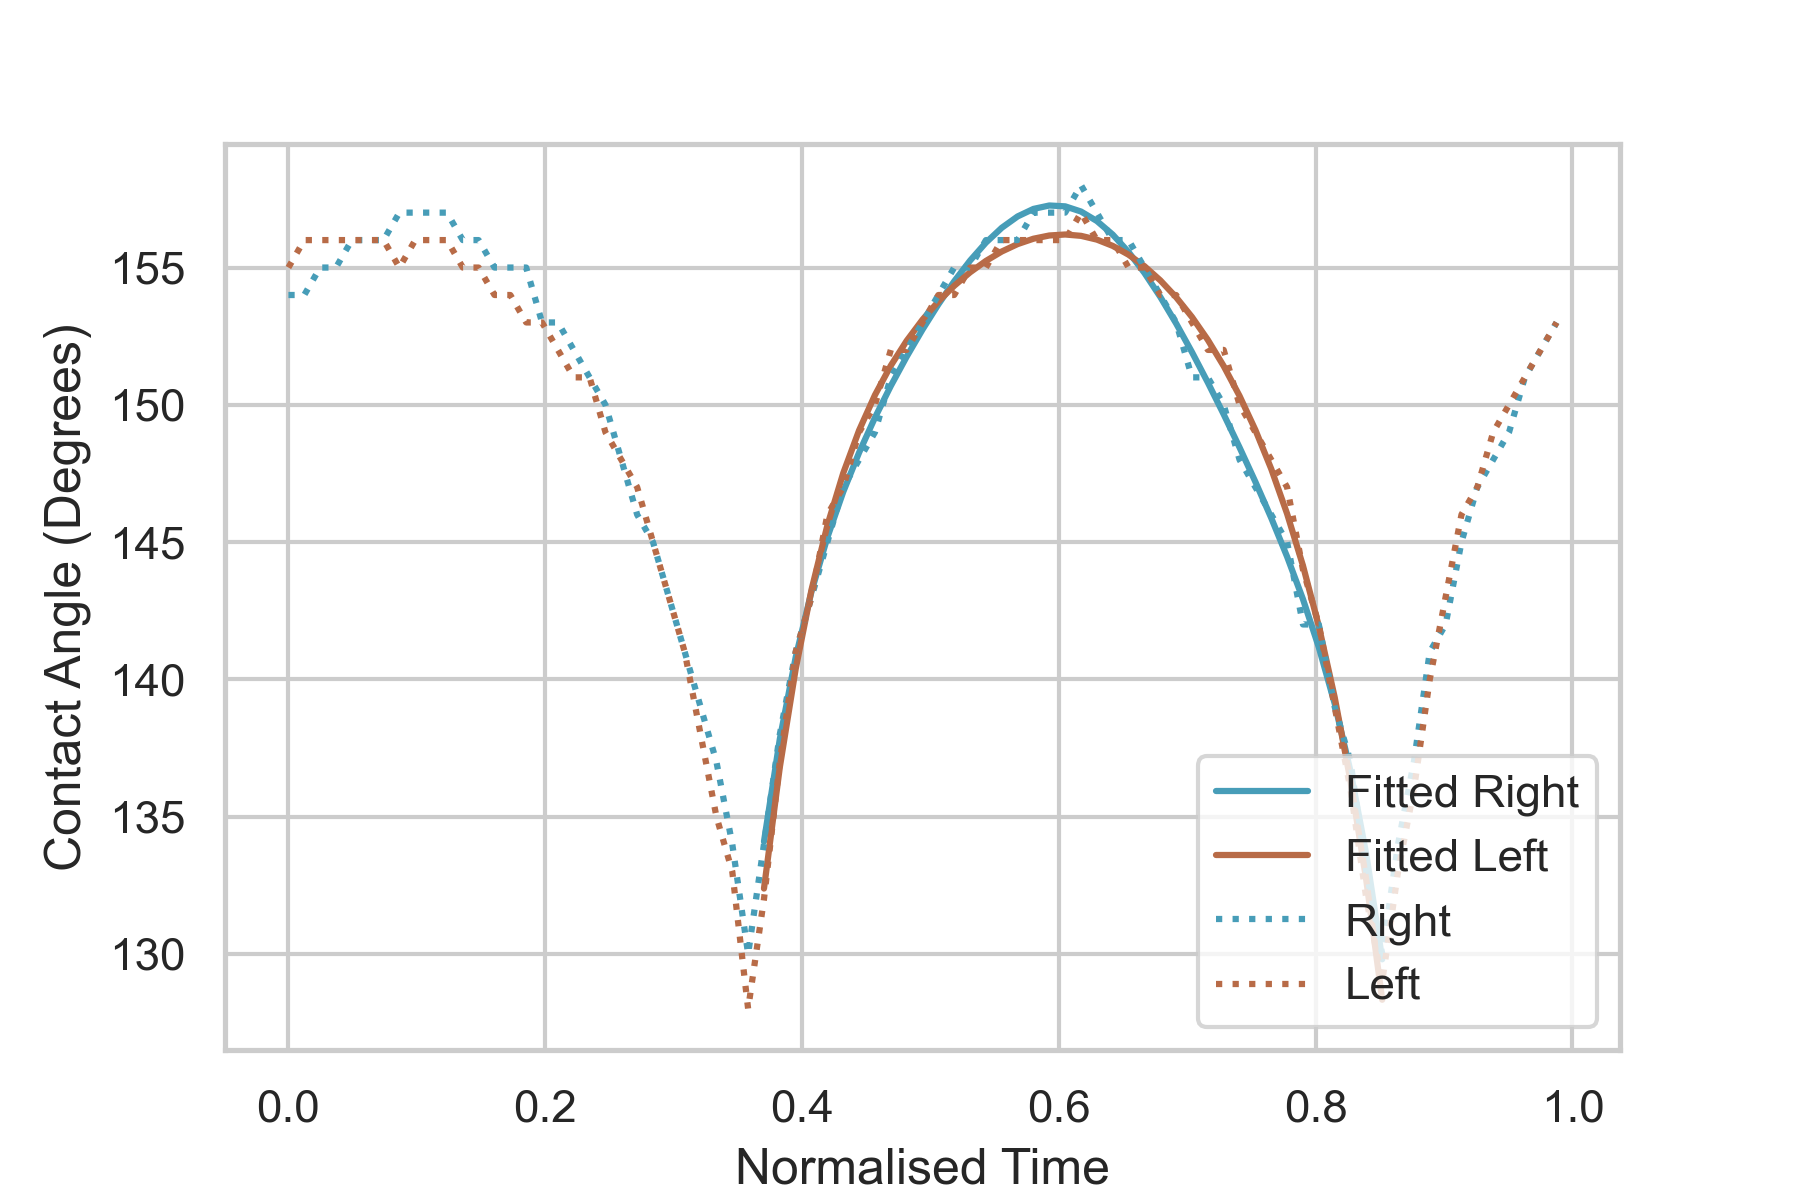
\includegraphics[width=0.5\textwidth]{Sections/Figures/B5055.png}
  \caption{B-50-5.5 slide hysteresis experiment showing Polynomial fitting}\label{Hyster}
\end{figure}
\subsection{Statistical Analysis Methodology}
The coefficient of determination ($R^2$) measured the fraction of the total variation in Y that is captured by the model. $R^2$ values were calculated to provide a quantitative measure of the polynomial's fit to the hysteresis data. In addition, the mean and standard deviation (SD) of static and advancing CA's were reported for each formulation. Comparison of the means amongst formulations were performed by one-way analysis of variance (ANOVA). ANOVA was used to evaluate whether there was any statistical evidence that the means of the sets of data differ using the F-distribution; therefore, the null hypothesis for this test was that all means were equal ($H_0: \mu_A = \mu_B =...$ ). During ANOVA, F-testing was conducted to test the underlying assumption of homoscedasticity as a preliminary step. If F > F crit  the null hypothesis was rejected and at least one of the means is statistically different'. This 'omnibus' testing (assuming a significant result) was followed up by multiple pair-wise category t-tests. The p-value was calculated to ascertain if there was a significant difference between specific individual groups. Statistical analysis between groups was primarily carried out on $\theta_A$ values as to not involve the uncertainty that is inherent from a metastable static droplet . 
\par Non-paired, two-sample unequal/equal variance (depending on the result of an initial F-test) t-testing was then performed between slides within the \emph{same} formulation to investigate the reproducibility of the dip-coating method. Factors that could affect these results include dipping speed, withdrawal speed, dipping angle etc. 
\par The null hypothesis here was that the two population’s of contact angles were the same ($H_0:\mu_1 = \mu_2$). The Alternative $H_1$ was that they were different due to non-reproducibility of the dip coating method. The inherent bias of slide selection was mitigated in-lab by choosing random slides for analysis. If the p-value was found to be above the significance level $\alpha = 0.05$, the null hypothesis was not rejected and there was not sufficient evidence to conclude non-reproducibility via dip-coating and the variance of angles that were measured in data occurred by chance or some other factor.
\subsection{Durability Testing Methodology}
'DVS Advantage' was used for \textbf{DVS testing} to determine the hygroscopicity of the coatings. 50mg of the optimised formulation samples were used due to their hydrophobic nature. A step change from 0\% RH to 90\% RH was used and ran for 750 mins to determine percentage change in mass. 
\par During \textbf{immersion testing} 2 slides of each formulation were placed into DI water in separate beakers. At 10 minute intervals up to 1 hour, the slides were taken out, dried with compressed nitrogen and static WCA recorded in triplicate. 

\begin{wrapfigure}{l}{0.17\textwidth}
\centering
    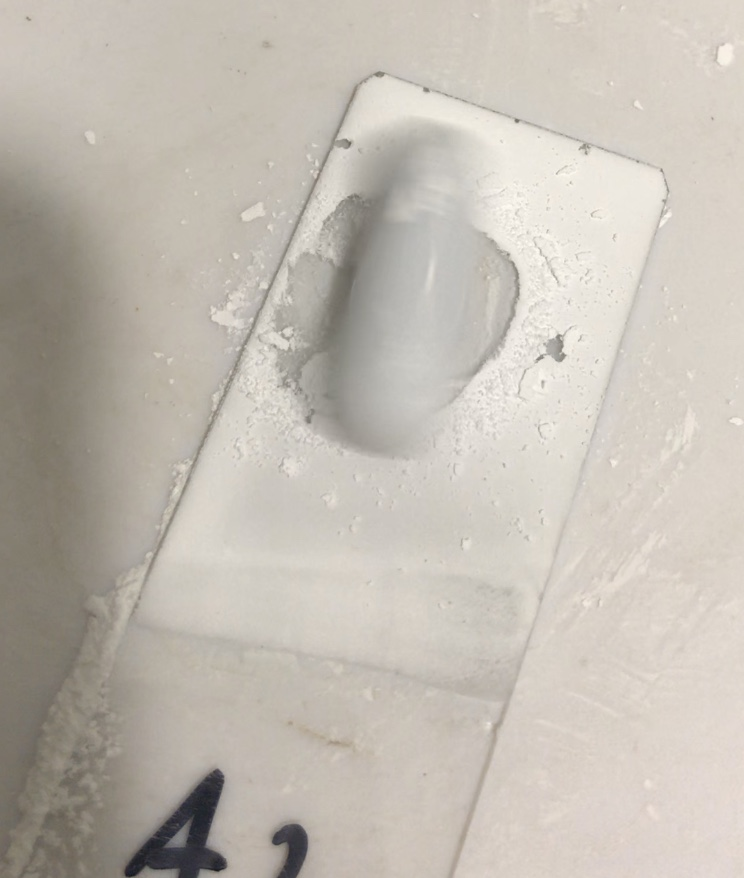
\includegraphics[width=0.1\textwidth]{Sections/Figures/MechanicalSetup.jpg}
\centering
  \caption{Stirrer causing surface mechanical abrasion}
  \label{abrasion_method}
\end{wrapfigure}

\par The qualitative \textbf{mechanical abrasion method} tested physical robustness of prepared coatings on the glass substrate. The rotation speed of a 2cm stirrer bead was kept constant at 150rpm and the time for glass to be first seen recorded, as in Figure \ref{abrasion_method}. This was repeated for 2 slides and the average determined. A 'Veho  VMS-004 microscope camera' capable of 20-400x magnification was used to take images of the area of abrasion.
\par The \textbf{outdoor test} aimed to investigate the change in film characteristics due to rain droplets and higher RH than indoors (\cite{syafiq_vengadaesvaran_ahmed_rahim_pandey_bushroa_ramesh_ramesh_2020}). 2 slides of each formulation had their static WCA measured before being placed outside on the window sill in SW7. Temperature and RH were monitored from BBC Weather for 5 days and the static WCA measured after being blown dry with compressed N$_2$. 


